\begin{center}
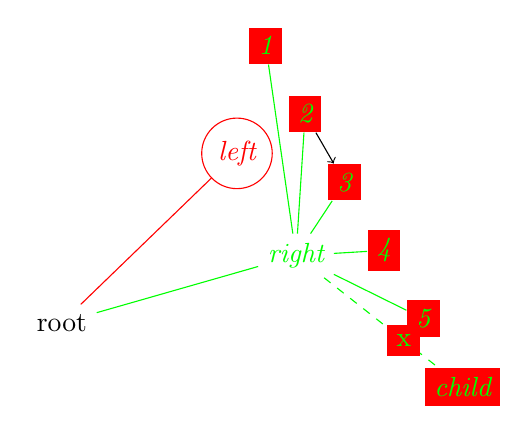
\begin{tikzpicture}
[
	level 2/.style 			=
	{
		sibling distance	= 10mm,
		level distance 		= 10mm,
		nodes 				= {fill = red}
	},
	every child node/.style	= {font = \itshape},
]


\node {root}
[
	grow'			= 30, % in degrees. ' reverses the order of the children.  
	green,
	level distance	= 30mm,
] % these apply to all children (if not overridden at the beginning)
child
[red] % this apply just to this child
{
	node [circle, draw] {left}
}
child
{
	node {right}
	child foreach \name in {1,...,5}
	{
		node (\name) {\name}
	}
	child
	{
		node {child}
		edge from parent [dashed] node [pos = 0.7] {x}
	}
};

\draw [->] (2) -- (3);

\end{tikzpicture}
\end{center}
